\chapter{Análisis de resultados}

Este capítulo presenta un estudio secuencial de los resultados, comenzando por la ejecución y evaluación de los algoritmos base que establecen los parámetros iniciales del modelo. En primer término, se implementa y analiza el algoritmo sin ponderación de zonas, que ofrece una línea base de rendimiento al tratar todas las áreas del campo con igual importancia. A continuación, se examina el comportamiento del algoritmo con ponderación uniforme, donde se asignan pesos estándar a cada zona, permitiendo una primera aproximación a las diferencias espaciales.

Una vez establecidas estas referencias iniciales, la investigación avanza hacia un análisis más granular. Se estudia el rendimiento colectivo de los equipos, examinando su influencia diferencial en las distintas zonas del campo, revelando patrones espaciales asociados al éxito deportivo. Este enfoque macro complementa el posterior análisis individual de jugadores mediante mapas de calor, que cuantifican la participación y efectividad de cada futbolista en áreas específicas.

La fase culminante aplica dos algoritmos genéticos que optimizan dinámicamente la ponderación zonal, contrastando sus resultados con los modelos base iniciales. Esta estructura metodológica, de lo general a lo particular, y de los modelos simples a los complejos, permite una validación rigurosa del sistema, demostrando cómo la ponderación inteligente de zonas mejora la capacidad predictiva respecto a los enfoques no ponderados.

El capítulo no solo compara la eficacia de cada método, sino que revela computacionalmente qué regiones del campo resultan más decisivas, proporcionando insights valiosos para la toma de decisiones técnicas. Esta progresión analítica garantiza una comprensión profunda de los factores espaciales que influyen en el rendimiento futbolístico.

\section{Algoritmo sin pesos}
La ejecución del algoritmo sin zonas, explicado en el capítulo anterior, es la siguiente:

\begin{figure}[H]
    \centering
    
\includegraphics[width=1.0\textwidth]{plantilla-TFG-ETSIIT/doc/imagenes/Ejecucion_simple.png}
    \caption{Ejecución algoritmo sin pesos}
    \label{fig:etiqueta-imagen}
\end{figure}

Al ejecutar el modelo sobre todos los partidos de la base de datos, se obtiene una precisión del 36,14\%, un valor relativamente bajo si se considera que existen únicamente tres posibles resultados en un partido: victoria local, victoria visitante o empate. Esto implica que la predicción se aproxima al azar, donde cada resultado tendría una probabilidad cercana al 33,3\%.


\section{Algoritmo con pesos}
La ejecución del algoritmo con zonas, el cual también ha sido explicado en el capítulo anterior, muestra:

\begin{figure}[H]
    \centering
    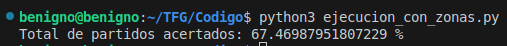
\includegraphics[width=1.0\textwidth]{plantilla-TFG-ETSIIT/doc/imagenes/Ejecucion_con_zonas.png}
    \caption{Ejecución algoritmo con pesos}
    \label{fig:etiqueta-imagen}
\end{figure}

Al ejecutar este algoritmo sobre todos los partidos disponibles en la base de datos, se obtiene una precisión del 67,47\%, una mejora significativa respecto a enfoques anteriores. Aunque este porcentaje ya puede considerarse aceptable dentro del contexto de la predicción de resultados en fútbol, aún existe margen de mejora, especialmente mediante el ajuste fino de los pesos y la incorporación de técnicas más avanzadas.

\section{Rendimiento de los equipos}
Una funcionalidad adicional incorporada al algoritmo con pesos es que permite visualizar el dominio territorial de cada equipo en el terreno de juego, a partir de la suma total de acciones realizadas en cada zona. Esta representación se genera mediante la función 'representar\_mapa', que recibe como argumentos dos vectores correspondientes a la sumatoria total de cada equipo en las 24 zonas del campo.

La función produce un mapa dividido en dichas zonas, coloreando en rojo aquellas en las que predomina el equipo 1 y en azul las dominadas por el equipo 2. Además, se tiene en cuenta la simetría del campo para mantener una visualización coherente: independientemente de si el equipo es local o visitante, sus estadísticas se ajustan para que ambos ataquen siempre de izquierda a derecha en la representación. De este modo, si el equipo visitante tiene mayor presencia ofensiva, dicha superioridad se visualizará en las zonas de ataque habituales, pero con el color azul que lo identifica.

A continuación, se muestra un ejemplo aplicado al partido Villarreal - Las Palmas correspondiente a la temporada 2024/2025 de la liga española:

\begin{figure}[H]
    \centering
    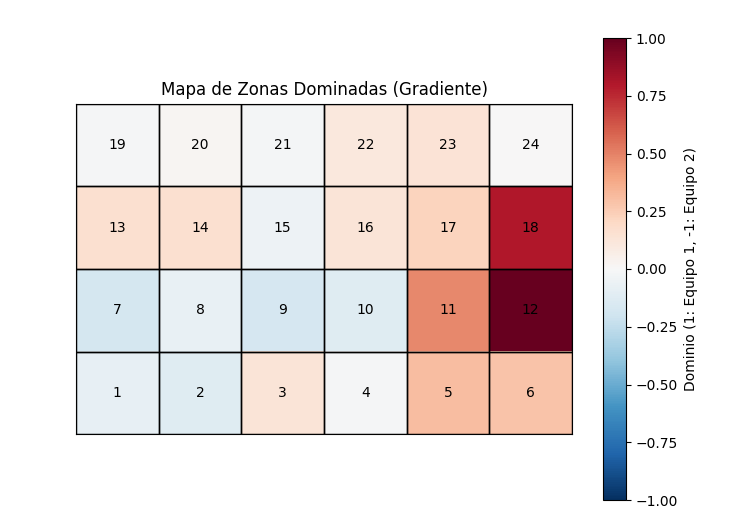
\includegraphics[width=0.6\textwidth]{plantilla-TFG-ETSIIT/doc/imagenes/Local_zonas_equipos.png}
    \caption{Mapa de zonas resultante del Villareal - Las Palmas}
    \label{fig:etiqueta-imagen}
\end{figure}

Como se puede observar en el mapa, el equipo local, el Villarreal, dominó claramente las zonas de ataque, especialmente aquellas más próximas a la portería rival. Este comportamiento es coherente con el resultado final del encuentro, que terminó con una victoria del Villarreal por 3-1. Este tipo de representación permite a los entrenadores obtener conclusiones tácticas relevantes: por ejemplo, se aprecia que el equipo visitante recibió una mayor presión por la banda derecha, incluso hasta la línea de fondo, lo que podría indicar la necesidad de reforzar la defensa en esa zona.
Del mismo modo, el cuerpo técnico del Villarreal podría interpretar este mapa como una confirmación del buen rendimiento colectivo, ya que su equipo apenas fue superado en ninguna zona del campo. En aquellos sectores donde el rival sí logró cierta presencia, las diferencias son mínimas, lo que podría considerarse como un equilibrio más que una desventaja.

A continuación, se analiza un ejemplo del Getafe - Las Palmas de la temporada 2024/2025 de la liga española, en el que el equipo visitante resultó vencedor:

\begin{figure}[H]
    \centering
    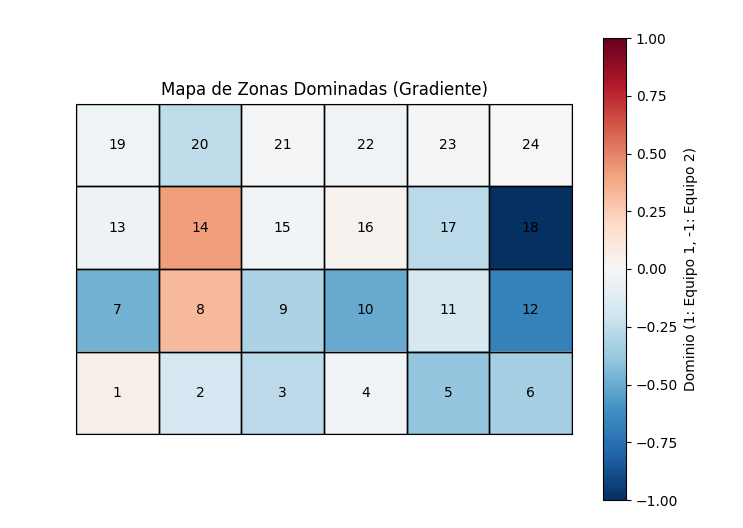
\includegraphics[width=0.7\textwidth]{plantilla-TFG-ETSIIT/doc/imagenes/Visitante_zonas_equipo.png}
    \caption{Mapa de zonas resultante del Getafe - Las Palmas}
    \label{fig:etiqueta-imagen}
\end{figure}

En este caso, puede apreciarse que el equipo visitante, representado en color azul, ha dominado en prácticamente todas las zonas del campo, con excepción de las dos zonas centrales de defensa. Esta distribución sugiere que el equipo local centró sus esfuerzos principalmente en tareas defensivas, concentrando su actividad en dichas áreas con el objetivo de contener los ataques rivales. Sin embargo, el amplio control territorial del equipo visitante indica un dominio generalizado del juego, lo que permite inferir que, a pesar de la resistencia defensiva local, no se logró frenar la ofensiva sostenida del adversario.

A continuación, se muestra un ejemplo correspondiente a un partido que finalizó en empate:

\begin{figure}[H]
    \centering
    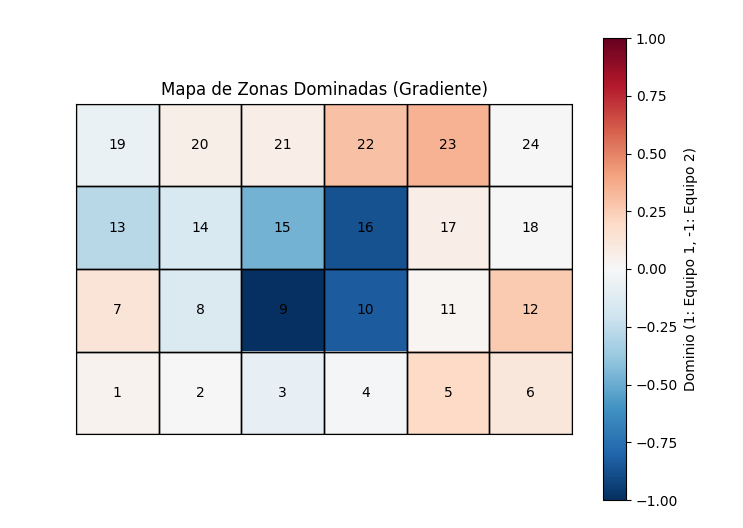
\includegraphics[width=0.7\textwidth]{plantilla-TFG-ETSIIT/doc/imagenes/Empate_zonas_equipos.png}
    \caption{Mapa de zonas resultante del Las Palmas - Sevilla}
    \label{fig:etiqueta-imagen}
\end{figure}

En el ejemplo correspondiente al encuentro entre Las Palmas y Sevilla, disputado durante la temporada 2024/2025 de la liga española, se observa que ninguno de los dos equipos logró dominar con claridad las zonas de ataque del adversario. No obstante, el equipo local mostró un mayor control en el centro del campo, aunque esta superioridad no fue suficiente para traducirse en una victoria.

Este tipo de visualización ofrece información valiosa para los entrenadores, ya que permite identificar con precisión las zonas del terreno donde el equipo necesita mejorar. A partir del análisis espacial del rendimiento, es posible extraer conclusiones tácticas relevantes y establecer líneas de actuación concretas de cara a futuros partidos.

\section{Rendimiento individual de cada futbolista}
En el análisis futbolístico, no solo es relevante estudiar el rendimiento colectivo del equipo, sino también el desempeño individual de cada jugador. Al igual que es posible acceder a la suma de acciones realizadas por el conjunto en cada zona del campo, este mismo análisis puede aplicarse a nivel individual. Esta perspectiva permite identificar qué futbolistas han tenido una participación más determinante durante el partido y cuáles han contribuido en menor medida.

La evaluación se basa en comparar la aportación del jugador en cada zona del campo con la suma total de las acciones del equipo en esa misma área. Al igual que en representaciones anteriores, los mapas se muestran siempre con el equipo atacando de derecha a izquierda, independientemente de si actúa como local o visitante. Para cada zona, si un jugador presenta una estadística igual o ligeramente inferior (hasta 0.2 puntos) respecto al total del equipo rival, se considera que ha tenido un papel relevante, aunque no diferencial, y se representa con un tono rojo claro. En cambio, si el jugador supera en una zona concreta la suma de las estadísticas del rival, dicha área se representa con un gradiente de color rojo, siendo más intenso en las zonas donde su impacto ha sido mayor. Todos los valores donde se ha sido predominante han sido normalizados en un rango de 0.0 a 0.1, excluyéndose de la normalización aquellos inferiores a -0.2, ya que no se consideran suficientemente significativos y se representan en el mapa de color blanco. 

A continuación, se muestran algunos mapas de calor correspondientes al encuentro entre Real Madrid F y Valencia F, perteneciente a la primera división femenina de España, con el objetivo de ilustrar esta metodología aplicada al análisis individual.

\begin{figure}[H]
    \centering
    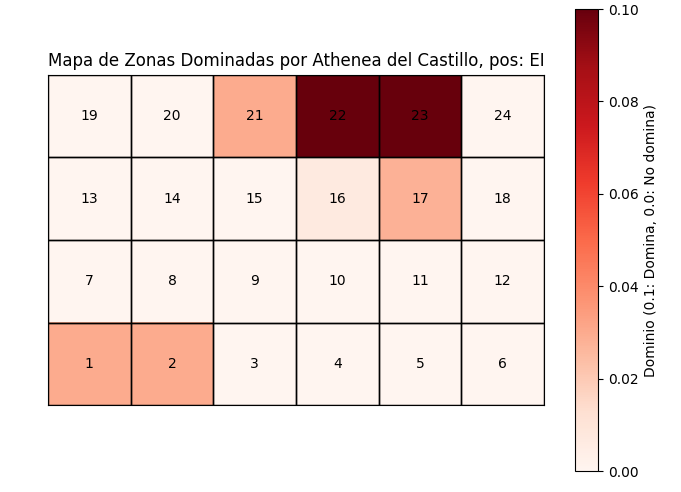
\includegraphics[width=0.7\textwidth]{plantilla-TFG-ETSIIT/doc/imagenes/futbolista_mapa_1.png}
    \caption{Mapa de influencia de Athenea de Castillo}
    \label{fig:etiqueta-imagen}
\end{figure}

Como se puede observar, esta futbolista que juega como extrema izquierda, dominó en las áreas relativas a su posición (17, 21, 22, 23), por lo que se puede deducir que fue capaz de desestabilizar a la defensa rival en esas zonas.

A continuación, se presenta el mapa de calor de la extrema izquierda que entró como sustituta de la futbolista que acabamos de ver:

\begin{figure}[H]
    \centering
    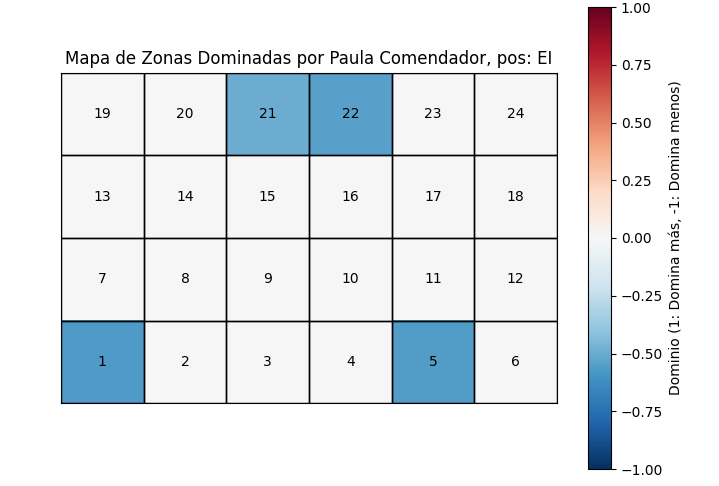
\includegraphics[width=0.7\textwidth]{plantilla-TFG-ETSIIT/doc/imagenes/Futbolista_mapa_3.png}
    \caption{Mapa de influencia de Paula Comendador}
    \label{fig:etiqueta-imagen}
\end{figure}

Como se observa, esta futbolista no fue tan dominante en las áreas relativas a su posición; de hecho, la extrema titular domina en más zonas y con más intensidad que ella. Esta información puede ser de gran utilidad para el entrenador a la hora de comparar futbolistas y tomar decisiones respecto a las alineaciones.

A continuación, se presenta el mapa de calor de una jugadora que desempeña el rol de lateral derecha. Recordemos que las zonas en rojo reflejan que las estadísticas de la futbolista en el partido superan en su totalidad a las del equipo rival en esa zona:

\begin{figure}[H]
    \centering
    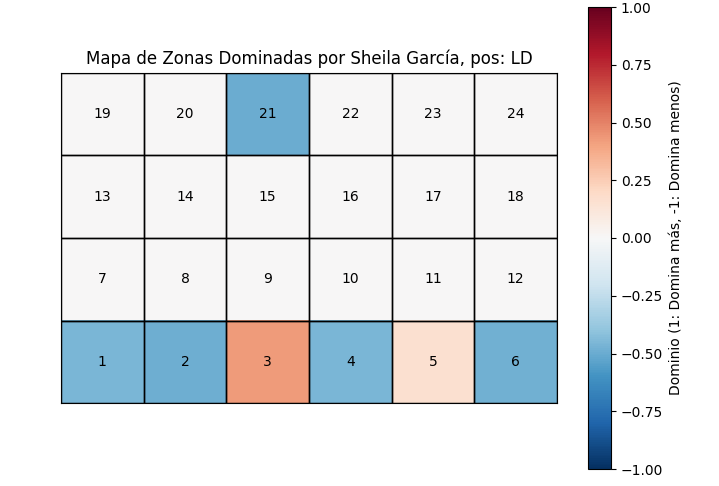
\includegraphics[width=0.7\textwidth]{plantilla-TFG-ETSIIT/doc/imagenes/Futbolista_mapa_2.png}
    \caption{Mapa de influencia de Sheila García}
    \label{fig:etiqueta-imagen}
\end{figure}

Como se aprecia en la imagen, esta futbolista fue claramente diferencial en su banda, ya que tiene una mayor intensidad en las zonas (1, 2, 3, 4 y 6), dominando casi completamente la banda derecha.

A continuación, se presenta un último ejemplo correspondiente a una defensa central en el encuentro entre Barcelona F y Athletic Club de Bilbao F:

\begin{figure}[H]
    \centering
    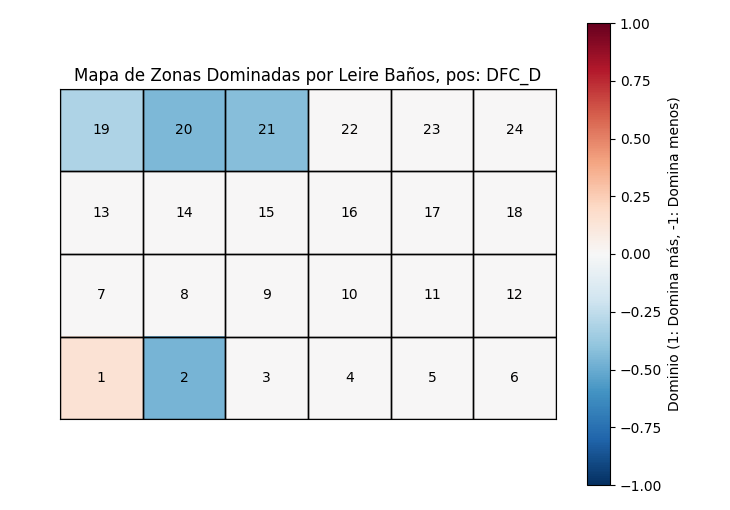
\includegraphics[width=0.7\textwidth]{plantilla-TFG-ETSIIT/doc/imagenes/futbolista_mapa_4.png}
    \caption{Mapa de influencia de Leire Baños}
    \label{fig:etiqueta-imagen}
\end{figure}

En este partido, se puede inferir que la defensa central por la derecha tuvo un desempeño deficiente, dado que no logró imponerse en las zonas centrales de la defensa, y sólo mostró cierta efectividad en los laterales. Esta situación podría llevar al entrenador a concluir que la jugadora se vio obligada a salir de su posición habitual para brindar apoyo defensivo a las laterales, en especial al lateral izquierdo.

Estas interpretaciones son ejemplos de cómo un entrenador puede analizar distintas situaciones tácticas del juego, tales como coberturas, presión alta o ataques por las bandas. Asimismo, este análisis puede profundizarse para comprender el estilo de juego del rival. En definitiva, esta técnica ofrece una herramienta valiosa para que el cuerpo técnico prepare el partido de manera más efectiva.

\section{Algoritmos genético}
En esta sección se describe el proceso de ejecución de los algoritmos genéticos implementados para el análisis y predicción del rendimiento en los partidos. Se detallan los parámetros configurados, las etapas de evolución del algoritmo y la forma en que se manejan los datos para obtener resultados óptimos. 

Para poder explorar las distintas soluciones del problema, y para asegurarnos de que nos quedamos con la mejor, se va a ejecutar varias veces combinando los datos:

\begin{itemize}
    \item Población: El de tamaño de la población será de 40 u 80.
    \item El número de iteraciones que hace el algoritmo será de 20, 40 u 80.
    \item La tasa de mutación será de 1 ó 0.9.
\end{itemize}

Para llevar a cabo la ejecución, inicialmente se aplicará el algoritmo con una población de 40 individuos, 20 iteraciones y una tasa de mutación de 1. A continuación, se repetirá el proceso modificando únicamente la tasa de mutación a 0.9, y así sucesivamente hasta cubrir todas las combinaciones posibles. Dado que cada ejecución puede prolongarse durante varias horas, también se ha considerado relevante registrar el tiempo que tarda cada proceso.

Con el fin de garantizar la fiabilidad de los resultados y minimizar el impacto de la aleatoriedad, lo ideal sería ejecutar cada combinación 30 veces. Sin embargo, debido a limitaciones temporales, se ha optado por realizar cinco ejecuciones por combinación, lo que asegura un nivel mínimo de confianza. En el análisis de resultados no se mostrarán todas las tablas individuales, sino que se presentarán las medias obtenidas de las cinco ejecuciones junto con sus correspondientes desviaciones típicas.

\begin{table}[H]
\centering
\caption{Resultados del algoritmo genético para diferentes configuraciones}
\label{tab:resultados_algoritmo}
\begin{tabular}{|c|c|c|c|c|c|}
\hline
\textbf{Población} & \textbf{Generaciones} & \textbf{Cruzamiento} & \textbf{Mutación} & \textbf{Precisión (\%)} & \textbf{ejecución (min)} \\
\hline
40 & 20 & 1 & 1/48 & $85.02 \pm 0.67$  & 10\\
40 & 20 & 0.9 & 1/48 & $84.32 \pm 1.43$ & 10 \\
40 & 40 & 0.9 & 1/48 & $83.34 \pm 2.46$ & 19 \\
40 & 40 & 1 & 1/48 & $85.02 \pm 0.65$ & 19 \\

80 & 20 & 0.9 & 1/48 & $84.78 \pm 0.65$ & 19\\
40 & 20 & 1 & 1/48 & $85.98 \pm 1.07$ & 19 \\
40 & 80 & 1 & 1/48 & $85.5 \pm 1.2$& 36 \\
40 & 80 & 0.9 & 1/48 & $84.3 \pm 3.39$ & 36 \\

80 & 40 & 0.9 & 1/48 & $86.46 \pm 0.53$ & 36\\
40 & 40 & 1 & 1/48 & $85.98 \pm 0.65$ & 36 \\
80 & 80 & 1 & 1/48 & $86.94 \pm 0.53$ & 69 \\
80 & 80 & 0.9 & 1/48 & $86.46 \pm 0.53$ & 69 \\

\hline
\end{tabular}
\end{table}

Como se puede ver en la tabla, la mejor combinación es la de 80 individuos, 80 generaciones y tasa de cruzamiento de 1, con una precisión del 86,94\% y con una desviación típica de 0,53\%. Vamos a ver un gráfico de la evolución del algoritmo con esos parámetros.

\begin{figure}[H]
    \centering
    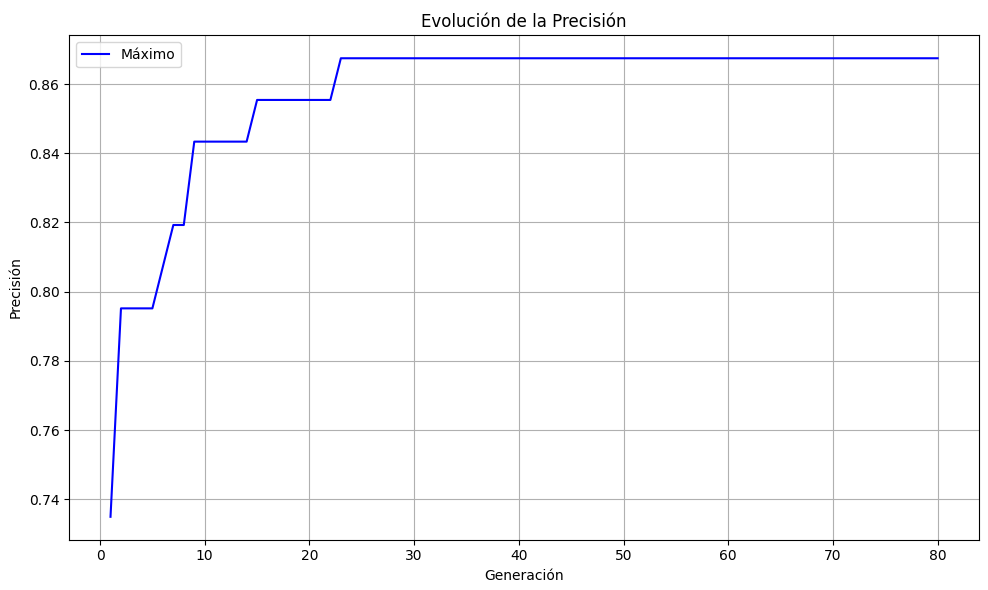
\includegraphics[width=1.0\textwidth]{plantilla-TFG-ETSIIT/doc/imagenes/Precision_gen.png}
    \caption{Gráfico algoritmo genético}
    \label{fig:etiqueta-imagen}
\end{figure}

Como se puede ver en el gráfico, el algoritmo evoluciona muy rápido, sin embargo, se estanca a partir de la generación 24. Los vectores que ha dado como resultado han sido los siguientes:

\begin{figure}[H]
    \centering
    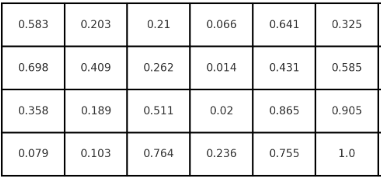
\includegraphics[width=0.7\textwidth]{plantilla-TFG-ETSIIT/doc/imagenes/Ataque_genetico.png}
    \caption{Vector de ataque genético}
    \label{fig:etiqueta-imagen}
\end{figure}

\begin{figure}[H]
    \centering
    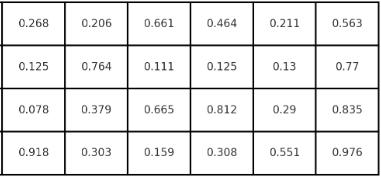
\includegraphics[width=0.7\textwidth]{plantilla-TFG-ETSIIT/doc/imagenes/Defensa_genetico.png}
    \caption{Vector de defensa genético}
    \label{fig:etiqueta-imagen}
\end{figure}

Como se puede observar, el vector de ataque incrementa a medida que el equipo avanza hacia el área rival, mientras que el vector de defensa se intensifica al retroceder hacia la propia. No obstante, existen ciertos valores atípicos, producto de la aleatoriedad inherente al fútbol, que no siguen este patrón. Aun así, es posible identificar una tendencia general. Además, se evidencia que la zona central del campo tiende a recibir menor atención estratégica en comparación con las áreas cercanas a las porterías.

\section{Algoritmo genético con $\delta$}
Para intentar que la predicción sea lo más precisa posible, vamos ahora a añadir al vector de pesos a $\delta$, que es la variable que representa en qué momento cortar para decidir si gana uno, otro o hay empate. Hasta ahora, esta variable había sido añadida a mano como 2, es decir, si:

\begin{itemize}
    \item $Score global > 2$, gana local
    \item $Score global < -2$, gana visitante
    \item empate en caso contrario
\end{itemize}

Ahora el algoritmo genético, aparte de definir los vectores de ataque y defensa para las ponderaciones de las zonas del campo, también va a decidir esta variable. La configuración del algoritmo es igual a la que se ha explicado antes, excepto para la tasa de mutación, que al añadir un nuevo valor al vector ha pasado a ser de 1/49. El objetivo es comparar técnicas y ver cuál es más rentable en cuanto a precisión y recursos.

Los distintos valores con los que se va a probar son los mismos que antes, se ha ejecutado un total de 5 veces y se ha calculado la media de cada combinación y su desviación típica.

\begin{table}[H]
\centering
\caption{Resultados del algoritmo genético con $\delta$ para diferentes configuraciones}
\label{tab:resultados_algoritmo}
\begin{tabular}{|c|c|c|c|c|c|}
\hline
\textbf{Población} & \textbf{Generaciones} & \textbf{Cruzamiento} & \textbf{Mutación} & \textbf{Precisión (\%)} & \textbf{ejecución (min)} \\
\hline
40 & 20 & 1 & 1/49 & $83.58 \pm 1.07$  & 13\\
40 & 20 & 0.9 & 1/49 & $83.6 \pm 1.03$ & 13 \\
40 & 40 & 0.9 & 1/49 & $83.58 \pm 0.65$ & 23 \\
40 & 40 & 1 & 1/49 & $85.02 \pm 1.37$ & 23 \\

80 & 20 & 0.9 & 1/49 & $85.5 \pm 1.47$ & 24\\
40 & 20 & 1 & 1/49 & $85.02 \pm 1.37$ & 24 \\
40 & 80 & 1 & 1/49 & $85.04 \pm 2.21$& 41 \\
40 & 80 & 0.9 & 1/49 & $84.78 \pm 1.37$ & 41 \\

80 & 40 & 0.9 & 1/49 & $86.22 \pm 0.65$ & 41\\
40 & 40 & 1 & 1/49 & $86.94 \pm 0.53$ & 41 \\
80 & 80 & 1 & 1/49 & $86.96 \pm 0.58$ & 86 \\
80 & 80 & 0.9 & 1/49 & $87.2 \pm 1.38$ & 86 \\

\hline
\end{tabular}
\end{table}

Como se puede apreciar, la mejor combinación es la de 80 individuos, 80 generaciones y tasa de cruzamiento 0.9 con una precisión del 87,2\% y una desviación típica de 1,38\%. El gráfico al ejecutarlo es el siguiente:

\begin{figure}[H]
    \centering
    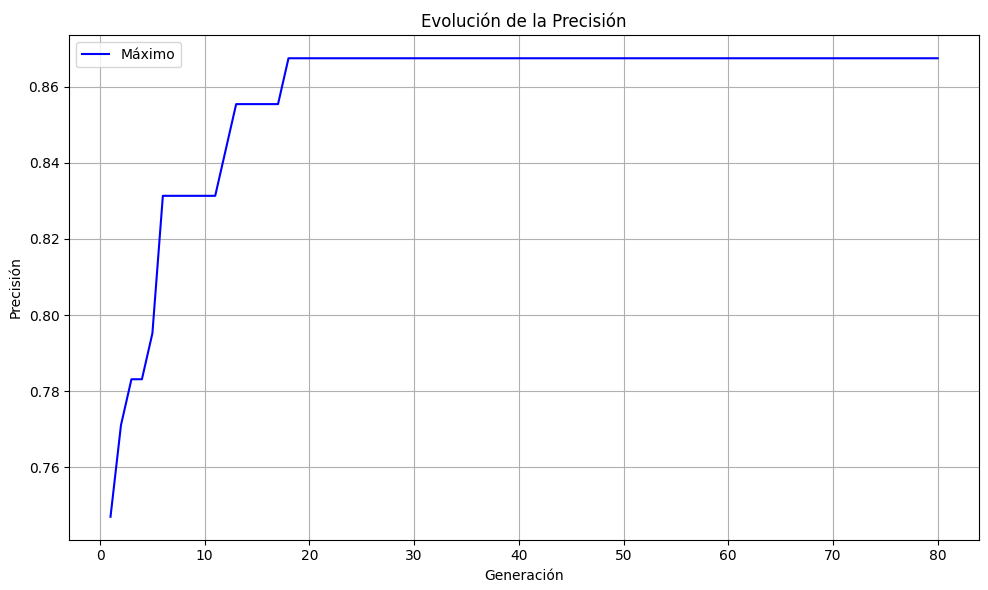
\includegraphics[width=0.7\textwidth]{plantilla-TFG-ETSIIT/doc/imagenes/Precision_delta.png}
    \caption{Grafico algoritmo genético}
    \label{fig:etiqueta-imagen}
\end{figure}

El gráfico es muy parecido al anterior, empieza evolucionando rápido, sin embargo, a partir de la generación 18 se estanca y no consigue avanzar más. Los vectores resultado son:

\begin{figure}[H]
    \centering
    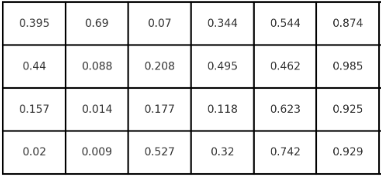
\includegraphics[width=0.7\textwidth]{plantilla-TFG-ETSIIT/doc/imagenes/Ataque_gen_delta.png}
    \caption{Vector de ataque genético con $\delta$}
    \label{fig:etiqueta-imagen}
\end{figure}

\begin{figure}[H]
    \centering
    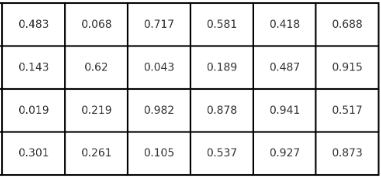
\includegraphics[width=0.7\textwidth]{plantilla-TFG-ETSIIT/doc/imagenes/Defensa_gen_delta.png}
    \caption{Vector de defensa genético con $\delta$}
    \label{fig:etiqueta-imagen}
\end{figure}

Los resultados de los vectores muestran un comportamiento similar al anterior: se otorga mayor relevancia a las áreas cercanas a las porterías que al centro del campo, aunque persisten ciertos valores aleatorios derivados de la impredecibilidad inherente al fútbol. Para determinar al ganador, se ha establecido un valor de corte, que se corresponde con $\delta$ de 1.75, ligeramente inferior al fijado manualmente en análisis previos, pero dentro de un rango comparable.

\section{Simetría de zonas}
Resulta llamativo que en la sección 6.5, dedicada a la ejecución del algoritmo genético, los resultados obtenidos presenten una marcada asimetría. Esta podría deberse a diversos factores, como la aleatoriedad inherente al fútbol, la tendencia de algunos equipos a atacar preferentemente por una banda concreta o, simplemente, a una coincidencia puntual.

En cualquier caso, se ha considerado oportuno analizar qué ocurriría si se partiera de un mapa con zonas simétricas. Para ello, se calculó la media de las zonas simétricas de los vectores generados por el algoritmo genético, tanto en ataque como en defensa. Posteriormente, se simularon todos los partidos de la base de datos utilizando estos pesos promedio, y a continuación se presentan los resultados obtenidos.

\begin{figure}[H]
    \centering
    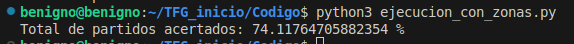
\includegraphics[width=0.7\textwidth]{plantilla-TFG-ETSIIT/doc/imagenes/zonas_simetricas.png}
    \caption{Ejecución con vectores simétricos}
    \label{fig:etiqueta-imagen}
\end{figure}

El resultado obtenido, del 74,11\%, mejora el rendimiento del sistema basado en la selección manual de pesos, aunque sigue siendo inferior al alcanzado por el algoritmo genético.

Puede considerarse un resultado aceptable en términos de predicción de partidos, si bien presenta una menor precisión en comparación con otros métodos más optimizados. Probablemente, la asimetría observada en los resultados esté relacionada con las dinámicas del fútbol moderno, en el que los equipos adoptan estrategias cada vez más complejas y tienden a concentrar su juego en determinadas zonas del campo, en lugar de mantener una distribución homogénea.

Por tanto, se valora la posibilidad de introducir ajustes adicionales en el modelo que permitan capturar mejor estas asimetrías, así como explorar variantes del algoritmo que integren este tipo de patrones estratégicos.

\section{Conclusión}
En términos generales, no se observa una diferencia significativa entre ambos algoritmos genéticos, lo que sugiere que el umbral utilizado para determinar el ganador a partir del puntaje global no resulta determinante. Esto probablemente se deba a que cada partido presenta valores variables, mayores o menores, en función de su desarrollo, y las puntuaciones de los equipos se adaptan a dichas circunstancias, evitando que exista una tendencia fija en el puntaje global.

Por otro lado, el porcentaje de acierto alcanzado, de $87.2 \pm 1.38$, es considerablemente alto para el contexto del fútbol, lo que permite afirmar con satisfacción que se ha logrado cumplir el objetivo principal planteado en este Trabajo de Fin de Grado.